\documentclass{ximera}

%\addPrintStyle{..}

\newcommand{\ul}[1]{#1}

\begin{document}
	\author{Bart Lambregs}
	\xmtitle{Verschillende soorten krachten}{}
    \xmsource\xmuitleg



\section*{Herhaling en uitbreiding soorten krachten}

Een kracht is een interactie tussen twee voorwerpen. 
Wanneer een eerste voorwerp A een kracht uitoefent op een ander voorwerp B, dan is een bepaalde uitwerking het mogelijk gevolg. 
Deze uitwerking kan \textbf{statisch (elastisch en/of plastisch)} zijn (vervorming), maar ook \textbf{dynamisch} (verandering van bewegingstoestand, in één woord: versnelling).

De meeste krachten zijn \textbf{contactkrachten}, dan is er rechtstreeks contact tussen de twee voorwerpen. 
Bij \textbf{veldkrachten} is geen rechtstreeks contact nodig en is er sprake van een krachtveld. 
De veldkrachten zijn: gravitatiekracht (of zwaartekracht) tussen massa's, elektromagnetische kracht tussen ladingen (Coulomb- en Lorentzkracht), sterke kernkrachten tussen quarks en de zwakke wisselwerking die in theorie mogelijk is tussen alle fundamentele deeltjes. 
Alle andere krachten zijn bijgevolg contactkrachten.

De grootheid kracht is een vector, ze heeft een richting, zin en grootte. 
De grootte van de kracht heeft als eenheid de Newton \SI{}{\newton}. 
Bij een contactkracht grijpt de kracht aan op de plaats(en) waar er contact is. 
Bij een veldkracht grijpen er in feite vele kleine veldkrachten aan op de betrokken deeltjes van gans het voorwerp. 
Voor de eenvoud vatten we die samen tot één kracht. 
Tenslotte laten we voor het gebruiksgemak meestal \textbf{alle krachten op een voorwerp aangrijpen in het zwaartepunt van het voorwerp}.


\begin{image}[0.5\textwidth]
  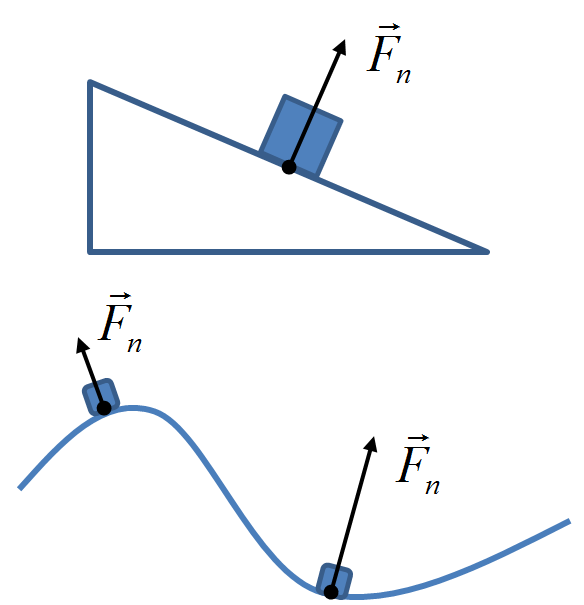
\includegraphics{toep_blok_helling}
\end{image}

Hoekan je achterhalen welke krachten op een voorwerp aangrijpen? 
Stel jezelf de vraag: ``Wat duwt of trekt eraan?'' 
Bepaal de contactkrachten door na te gaan met welke voorwerpen er contact is en overloop dan de eventuele veldkrachten.

\section*{De normaalkracht (contactkracht)}


De normaalkracht is een kracht van een (meestal vlakke, maar soms ook gebogen) ondergrond op een voorwerp, meestal met de bedoeling het voorwerp te ondersteunen. 
De normaalkracht \({\overrightarrow{F}}_{n}\) staat altijd loodrecht op het grondvlak (net zoals de normale versnelling loodrecht staat op de snelheidsvector; ``normaal'' betekent in deze context nu eenmaal ``loodrecht''). 
Er is geen formule om de grootte van de normaalkracht uit te rekenen. 
De grootte ervan dient altijd bepaald te worden uit de toepassing van en het redeneren met de wetten van Newton. 
In sommige eenvoudige situaties kan het zijn dat \(F_{n} = F_{z}\), \textbf{maar dit is zeker niet altijd het geval! Enkel met behulp van de wetten van Newton is er uitsluitsel!}

\section*{De veerkracht (contactkracht)}
De veerkracht is een kracht die een uitgerekte of ingedrukte veer uitoefent op een voorwerp die met één van de uiteindes verbonden is.
Wanneer de veer onbelast is (m.a.w. niet uitgerekt of ingedrukt, maar gewoon ontspannen) dan heeft ze een rustlengte \(\mathcal{l}_{r}\). 
Bij belasting is de lengte \(\mathcal{l}\) verschillend van rustlengte \(\mathcal{l}_{r}\) en is er een uitrekking/indrukking, hetgeen met \(\mathcal{\mathrm{\Delta}l = l -}\mathcal{l}_{r}\) wordt weergegeven.
Bij zuiver elastische vervormingen (dit zijn niet al te grote vervormingen zodat bij ontspanning de veer uit zichzelf terug tot aan de rustlengte ontspant) geldt de wet van Hooke als formule voor de grootte van de veerkracht:
\(\mathbf{\ F}_{\mathbf{v}}\mathbf{= k \bullet}\left| \mathcal{\mathrm{\Delta}l} \right|\mathbf{\ }\).
Hierin is \(k\) de veerconstante uitgedrukt in \(\frac{N}{m}\). 
De waarde ervan is specifiek voor elke veer en is ook constant indien de veer enkel elastisch vervormt. 
Ze drukt uit hoeveel Newton kracht de veer zet per meter dat de veer is verlengd/verkort t.o.v. de rustlengte.
Ze zegt dus iets over de soepelheid of stijfheid van een veer.

\begin{image}
  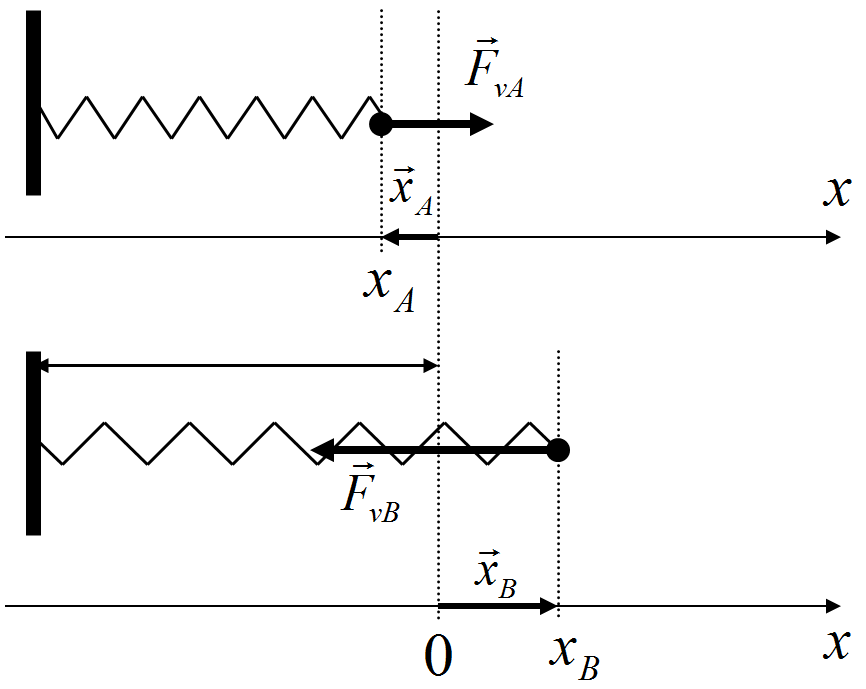
\includegraphics{toep_veer}
\end{image}

Het gebeurt dat voor het symbool \(\mathcal{\mathrm{\Delta}l}\) het symbool \(x\) gebruikt wordt. 
Dit is korter en dus eenvoudiger omdat de lengte van de veer ons meestal niet interesseert, enkel het verschil met de rustlengte. 
Dit zal in het vervolg van de cursus ook zo zijn. 
Meer nog, men kan voor de veerkracht ook een vectoriële formule opstellen indien men de uitrekking/indrukking van de veer als een uitwijkingsvector \(\overrightarrow{x}\) ziet die aangrijpt op de plaats van de rustlengte. Bijgevoegde figuren tonen dit voor een ingedrukte en uitgerekte veer. 
Er valt op dat de veerkracht telkens de tegengestelde zin heeft van de uitwijkingsvector, waardoor de vectoriële formule wordt:
\(\ {\ \overrightarrow{F}}_{v} = - k \bullet \overrightarrow{x}\ \). 
Descalaire getalcomponent (waarin met behulp van een gekozen x-as rekening wordt gehouden met de zin van de kracht) wordt dan:
\({\ F}_{v} = - k \bullet x\ \).

\[\mathcal{l}_{r}\]

\section*{De opwaartse stuwkracht in een vloeistof of Archimedeskracht}

\begin{image}  
  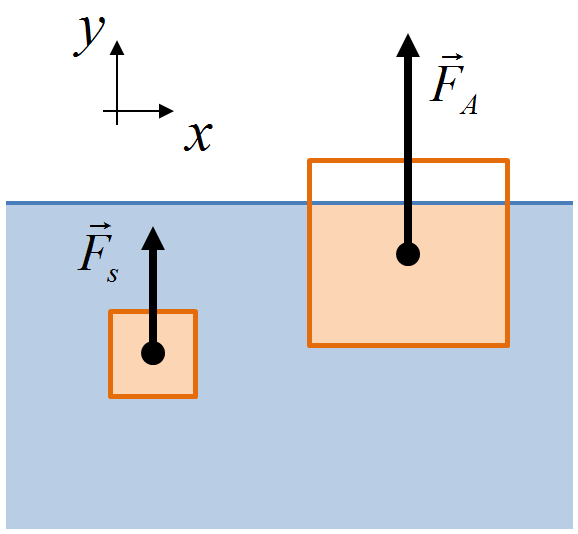
\includegraphics{toep_archimedes}
\end{image}


Eenvoorwerp dat volledig of gedeeltelijk ondergedompeld is in een vloeistof ondervindt vanwege de vloeistof een opwaartse stuwkracht verticaal omhoog. 
Deze kracht (van vloeistof op voorwerp) noemt men ook de Archimedeskracht. 
De verklaring ligt in het feit dat de hydrostatische druk onder het voorwerp groter is dan de druk boven het voorwerp. 
In feite is de Archimedeskracht dus de nettokracht van alle drukkrachten die de vloeistof op het voorwerp zet. 
Er kan proefondervindelijk en theoretisch aangetoond worden dat de grootte van deze kracht gelijk is aan die van de zwaartekracht op de verplaatste vloeistof (= wet van
Archimedes). 
Dit komt neer op:

\({\ F}_{s} = {\ F}_{A} = m_{vl} \bullet g = \rho_{vl} \bullet V_{verplaatst} \bullet g\)

Omdat de verplaatste vloeistof gelijk is aan het volume van het stuk voorwerp dat zich onder het vloeistofoppervlak bevindt, kan eveneens gezegd worden dat:

\({\mathbf{\ \ }\mathbf{F}}_{\mathbf{s}}\mathbf{=}{\mathbf{\ }\mathbf{F}}_{\mathbf{A}}\mathbf{=}\mathbf{\rho}_{\mathbf{vl}}\mathbf{\bullet}\mathbf{V}_{\mathbf{ond}}\mathbf{\bullet g\ }\)
met \(V_{ond}\) het ondergedompeld deel van het voorwerp. 

Om de grootte, richting en zin van de versnelling van een ondergedompeld voorwerp te bepalen, dient men de wetten van Newton toe te passen.
Hierin onderscheidt men een aantal gevallen:

\begin{itemize}
\item Zinken: \({\overrightarrow{a}}_{y}\) is naar beneden gericht (en
  \({\overrightarrow{F}}_{ry}\) ook, de neerwaartse krachten zijn samen
  sterker dan de opwaartse)
\item Stijgen: \({\overrightarrow{a}}_{y}\) is naar boven gericht (en
  \({\overrightarrow{F}}_{ry}\) ook, de opwaartse krachten zijn samen
  sterker dan de neerwaartse)
\item Zweven: voorwerp volledig ondergedompeld en \(a_{y} = 0\) (en dus is
  \(F_{ry} = 0\))
\item Drijven: voorwerp gedeeltelijk ondergedompeld en \(a_{y} = 0\) (en dus
  is \(F_{ry} = 0\))
\end{itemize}

Speciaal geval: Heel vaak werken op een ondergedompeld voorwerp slechts twee krachten, de Archimedeskracht (naar boven) en de zwaartekracht (naar onder) met bijbehorende formules:

\[{\ F}_{A} = \rho_{vl} \cdot V_{ond} \cdot g \]

\[ F_z = m_{vw} \cdot g = \rho_{vw} \cdot V_{vw} \cdot g \]

\begin{itemize}
\item
  Indien in dit geval het voorwerp \ul{volledig ondergedompeld} is, is
  \(V_{ond} = V_{vw}\) waardoor enkel de massadichtheden een verschil in
  grootte tussen de twee krachten kunnen opleveren, met als gevolg:
\end{itemize}

\[\rho_{vw} > \rho_{vl}\overset{}{\Rightarrow}zinken\ \ \ \ \ \ \rho_{vw} = \rho_{vl}\overset{}{\Rightarrow}zweven\ \ \ \ \ \ \rho_{vw} < \rho_{vl}\overset{}{\Rightarrow}stijgen\ (om\ nadien\ vermoedelijk\ te\ gaan\ drijven)\]

\begin{itemize}
\item
  Als het voorwerp \ul{gedeeltelijk ondergedompeld} is, dan is
  \(V_{ond} < V_{vw}\) en moet men ook met de volumes rekening houden om
  het gedrag te bepalen. Merk op dat in deze situatie bij drijven (=
  rustsituatie waarbij slechts een gedeelte van het voorwerp
  ondergedompeld is) moet gelden dat \({\ F}_{A} = {\ F}_{z}\).
\end{itemize}

\begin{image}
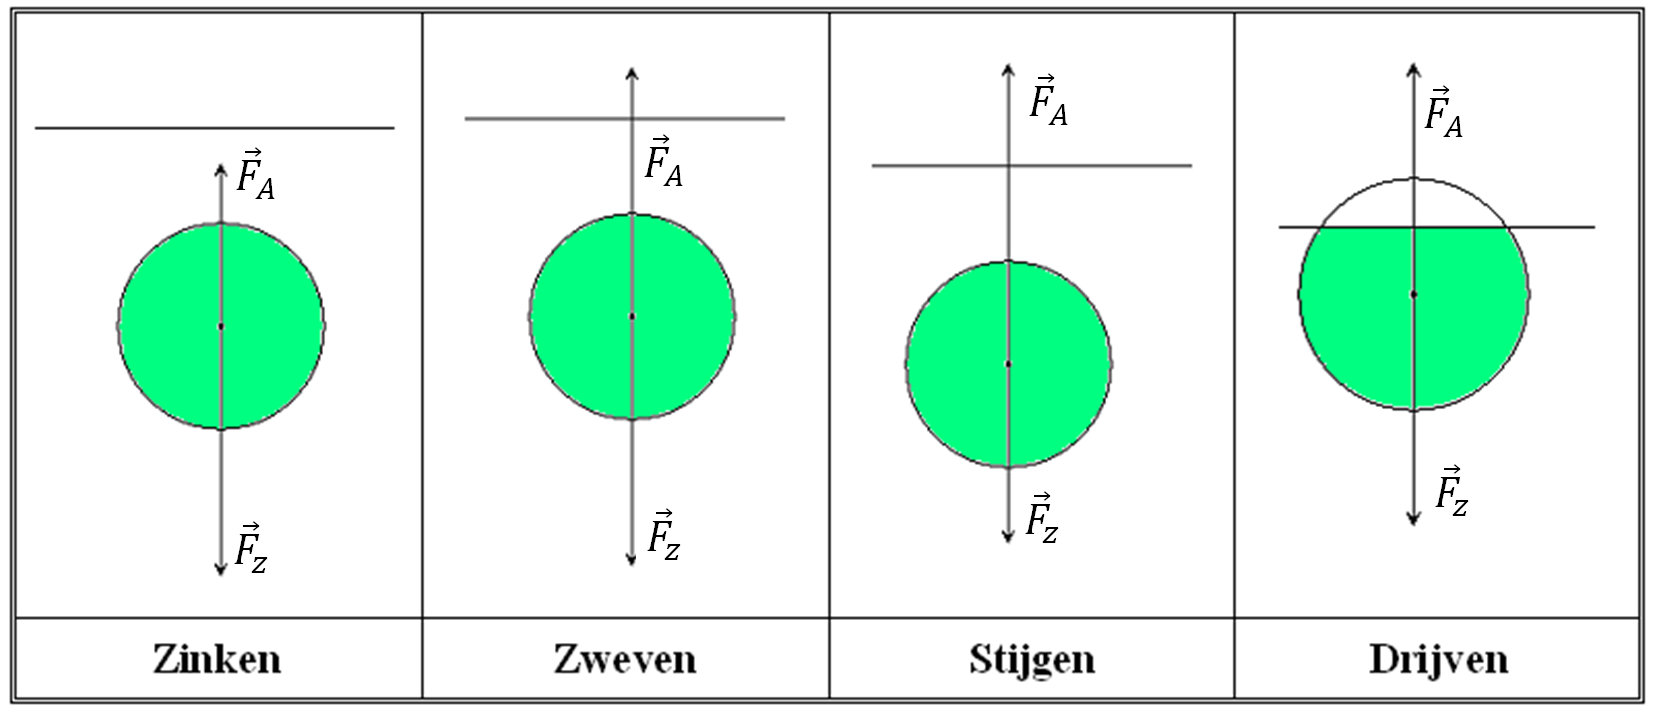
\includegraphics{toep_archimedes2}
\end{image}


Speciaal geval: ondergedompeld voorwerp ondervindt enkel \({\ \overrightarrow{F}}_{A}\) en \({\ \overrightarrow{F}}_{z}\). 
Het ondergedompeld volume is ingekleurd.

\section*{De gravitatiekracht of zwaartekracht (veldkracht)}

= aantrekkingskracht tussen massa's

\begin{image}
  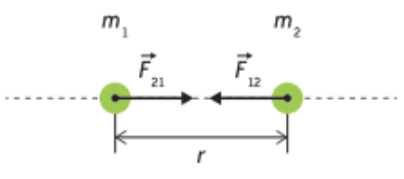
\includegraphics{toep_coulomb}
\end{image}

De \textbf{grootte} van de gravitatiekracht \({\overrightarrow{F}}_{G}\) tussen twee puntmassa's \(m_{1}\) en \(m_{2}\) met een afstand \(r\ \) tussenbeiden is gelijk is aan:

\[\mathbf{F}_{\mathbf{G}}\mathbf{= G \bullet}\frac{\mathbf{m}_{\mathbf{1}}{\mathbf{.}\mathbf{m}}_{\mathbf{2}}}{\mathbf{r}^{\mathbf{2}}}\ \text{met} \ G = 6,67 \bullet \SI{1e-11}{\newton\meter\squared\per\kilo\gram\squared} = gravitatieconstante\]

In realistische situaties bij voorwerpen met afmetingen is \(r\) de afstand tussen de zwaartepunten van die voorwerpen. 
Vaak valt het zwaartepunt samen met het midden van het voorwerp (zeker bij voorwerpen met homogene massaverdeling).

In de context van hemellichamen wordt gravitatiekracht vaak zwaartekracht genoemd. 
Dit verschilt enkel in benaming, maar beide benamingen weerspiegelen identiek hetzelfde krachtfenomeen. 
In het Engels of Frans bestaat er geen woord voor ``zwaartekracht'', zij kennen enkel \emph{gravity} of \emph{gravité}.

In een gravitatieveld \(\overrightarrow{g}\) is er een eenvoudigere formule:
\(\ {\overrightarrow{\mathbf{F}}}_{\mathbf{G}}\mathbf{=}{\overrightarrow{\mathbf{F}}}_{\mathbf{z}}\mathbf{= m \bullet}\overrightarrow{\mathbf{g}}\mathbf{\ }\)

Rond een hemellichaam met massa \(M\) geldt:
\(g = \frac{G \bullet M}{r²}\) 
Op het aardoppervlak, levert dit:
\(g_{A} = 9,81\frac{N}{kg} \approx 10\frac{N}{kg}\)


\section*{De elektrische kracht of Coulombkracht (veldkracht)}

= aantrekking- of afstotingskracht tussen elektrische ladingen

De \textbf{grootte} van de Coulombkracht \({\overrightarrow{F}}_{C}\)
(of elektrische kracht \({\overrightarrow{F}}_{e}\)) tussen twee
puntladingen \(q_{1}\) en \(q_{2}\) met een afstand \(r\ \)tussenbeiden
is gelijk is aan:

\[{\mathbf{F}_{\mathbf{C}}\mathbf{=}\mathbf{F}}_{\mathbf{e}}\mathbf{= k \bullet}\frac{\left| \mathbf{q}_{\mathbf{1}} \right|\mathbf{\bullet}\left| \mathbf{q}_{\mathbf{2}} \right|}{\mathbf{r}^{\mathbf{2}}}\ met\ k = 8,99 \bullet 10^{9}\frac{N \bullet m²}{C²} \approx 9,0 \bullet 10^{9}\frac{N \bullet m²}{C²}\]

\begin{image}
  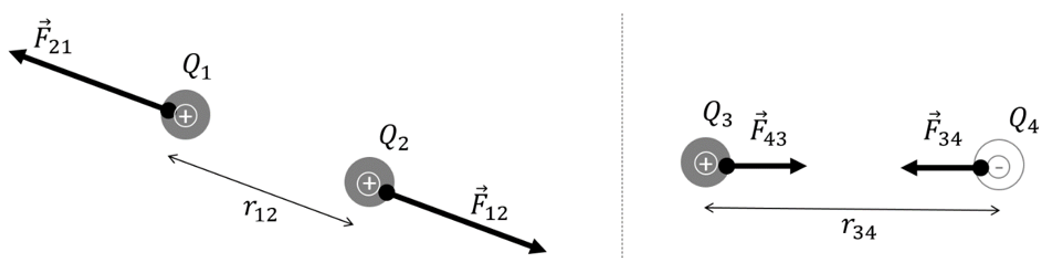
\includegraphics{toep_coulomb2}
\end{image}

In realistische situaties bij ladingen met afmetingen is r de afstand tussen de middelpunten van die ladingen.

In een elektrisch veld \(\overrightarrow{E}\) is er een eenvoudigere formule:
\(\ {\overrightarrow{\mathbf{F}}}_{\mathbf{C}}\mathbf{=}{\overrightarrow{\mathbf{F}}}_{\mathbf{e}}\mathbf{= q \bullet}\overrightarrow{\mathbf{E}}\mathbf{\ }\)
De grootte van \(\overrightarrow{E}\) kan in verschillende situaties bepaald worden naargelang het type veld. 
Meer details: zie leerstof 5\textsuperscript{de} jaar.


\section{De magnetische kracht of Lorentzkracht (veldkracht)}

= kracht op bewegende lading in een magnetisch veld (dat veroorzaakt wordt door andere bewegende ladingen)

De \textbf{grootte} van de Lorentzkracht \({\overrightarrow{F}}_{L}\) (of magnetische kracht \({\overrightarrow{F}}_{m}\)) op een lading \(q\) met snelheid \(\overrightarrow{v}\) die een hoek \(\alpha\) maakt met de magnetische veldsterkte \(\overrightarrow{B}\) waar de lading door vliegt is te berekenen met:

\[{\mathbf{F}_{\mathbf{L}}\mathbf{= F}}_{\mathbf{m}}\mathbf{= B \bullet}\left| \mathbf{q} \right|\mathbf{\bullet v \bullet}\mathbf{\sin}\mathbf{\alpha}\ met\ \alpha = hoek\ tussen\ \overrightarrow{B}\ en\ \overrightarrow{v}\]

Als vele ladingen samen een gemeenschappelijke driftsnelheid hebben door
een magneetveld hebben (vaak door een geleidende draad met lengte \(\mathcal{l}\)) beschouwt men dit als een stroom \(I\) in een magneetveld \(\overrightarrow{B}\). 
Dan wordt de formule:

\[{\mathbf{F}_{\mathbf{L}}\mathbf{= F}}_{\mathbf{m}}\mathbf{= B \bullet I}\mathcal{\bullet l \bullet}\mathbf{\sin}\mathbf{\alpha}\ met\ \alpha = hoek\ tussen\ \overrightarrow{B}\ en\ I\ \ (ook\ Laplacekracht\ genoemd)\]

\begin{image}
  % 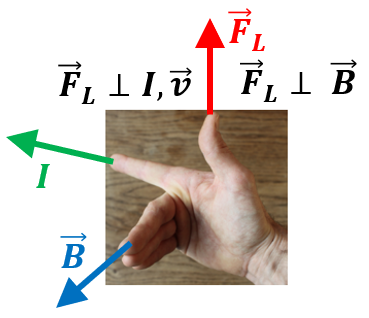
\includegraphics{toep_rechterhand}
  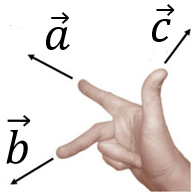
\includegraphics{rechterhandregel}
\end{image}

De richting en zin van \({\overrightarrow{F}}_{L}\) kan bepaald worden met de derde rechterhandregel waarin geredeneerd wordt met de conventionele stroomzin van de ladingen.

\emph{\textbf{Uitbreiding:} De Coulombkracht en de Lorentzkracht kunnen samengevat worden tot één elektromagnetische kracht, want beide gevallen gaan over kracht op een lading.}

\begin{quote}
\[{{\overrightarrow{\mathbf{F}}}_{\mathbf{em}}\mathbf{=}{\overrightarrow{\mathbf{F}}}_{\mathbf{C}}\mathbf{+}{\overrightarrow{\mathbf{F}}}_{\mathbf{L}}\mathbf{= q}\overrightarrow{\mathbf{E}}\mathbf{+ q}\overrightarrow{\mathbf{v}}\mathbf{\times}\overrightarrow{\mathbf{B}}\mathbf{= q}\left( \overrightarrow{\mathbf{E}}\mathbf{+}\overrightarrow{\mathbf{v}}\mathbf{\times}\overrightarrow{\mathbf{B}} \right)\mathbf{\ \ \ \ 
}}
\](\(\times is\ het\ symbool\ voor\ vectorieel\ product,\ zie\ externe\ cursussen\))
\end{quote}


\section*{De sterke kernkracht en zwakke wisselwerking (veldkrachten)}

De sterke kernkrachten tussen quarks zijn heel relevant voor de stabiliteit en samenhang van nucleonen in atoomkernen. 
Ze hebben echter geen relevantie in de stabiele macroscopische wereld. 
Enkel bij zeer kleine afstand tussen nucleonen (orde femtometer = 10\textsuperscript{-15} m) is deze kernkracht niet te verwaarlozen, binnen één atoomkern dus. 
De sterke kernkracht neemt met de afstand veel feller af in vergelijking met andere veldkrachten.

Bij de zwakke wisselwerking (of kernkracht) tussen fundamentele deeltjes is er een andere uitwerking dan gebruikelijk (niet statisch of dynamisch). 
In dit geval veranderen de deeltjes van aard. 
Ook dit fenomeen is in onze stabiele macroscopische wereld irrelevant omdat het net enkel gebeurt bij onstabiele deeltjes of atoomkernen.


\section*{De wrijvingskracht (contactkracht) (zie uitgebreid verhaal in boek FV p113-115)}

= weerstandskracht \({\overrightarrow{F}}_{w}\) op een voorwerp van een
medium of middenstof waarin of waartegen het zich bevindt

% \includegraphics[width=2.08889in,height=1.81111in,alt={E:\textbackslash School updated tot en met 27\_08\_2012\textbackslash Fysica 6de jaar\textbackslash Afbeeldingen\textbackslash wrijving.gif}]{media/image8.gif}\textbf{Schuifwrijvingskracht}
= weerstandskracht van een vlakke ondergrond op een voorwerp dat erop
steunt, evenwijdig met het vlak (en vaak tegen de zin van de beweging)

Verklaring schuifwrijving: een vlakke ondergrond is nooit perfect vlak!
Zie figuur.

Voor de \ul{schuif}wrijvingskracht \({\overrightarrow{F}}_{w}\) wordt vastgesteld dat\ldots{}

\begin{enumerate}
\item\ldots indien het voorwerp in rust is: \({\overrightarrow{F}}_{w}\) heeft die grootte en zin zodat \(F_{r} = 0\)
\item\ldots indien het voorwerp een rechtlijnige beweging maakt:
\end{enumerate}

De zin van \({\overrightarrow{F}}_{w}\) is tegen de zin van de beweging en de grootte van \({\overrightarrow{F}}_{w}\) is recht evenredig is met de grootte van de normaalkracht en tegelijk afhankelijk van hoe goed of slecht de materialen van het voorwerp en vlakke ondergrond over mekaar schuiven.

Er geldt dan: \(F_{w} = \mu \bullet F_{n}\) met \(\mu\) de schuifwrijvingsfactor of schuifwrijvingscoëfficiënt (op te zoeken in tabellen)

Bovenstaande omkaderde formule is dus de maximale waarde van de schuifwrijvingskracht, waardoor de formule beter te schrijven is als: \(F_{w,max} = \mu \bullet F_{n}\). 
Men kan overigens aantonen dat deze laatste formule ook klopt bij bewegingen die niet rechtlijnig zijn (zie verder voor voorbeelden). 
\textit{(zie ook animatie Hans Bekaert: ``wrijving'')}

\begin{enumerate}
\def\labelenumi{\alph{enumi})}
\setcounter{enumi}{2}
\item
  \ldots indien het voorwerp een ECB maakt: \({\overrightarrow{F}}_{w}\)
  heeft die grootte zodat
  \(F_{r} = m \bullet a = m \bullet \frac{v^{2}}{r} = m \bullet \omega ² \bullet r\)
\end{enumerate}

Bij het maken van een bocht (bijvoorbeeld ECB) is er in sommige gevallen schuifwrijvingskracht die bijdraagt tot de middelpuntzoekende kracht. 
Bij bijna alle vervoerswijzen over een vlakke weg doet dit zich voor (zoals met de wagen, met de fiets en zelfs te voet!). 
Er dient wel rekening gehouden te worden met het feit dat de schuifwrijvingskracht in grootte beperkt is tot \(F_{w,max} = \mu \bullet F_{n}\) waardoor er een gevaar bestaat dat de beoogde bocht niet gemaakt kan worden! 
In dit geval spreekt men van slippen en ``uit de bocht vliegen''. 
Zie oefeningen voor concrete gevallen.


%%TODO%% \includegraphics[width=3.08403in,height=2.31111in,alt={E:\textbackslash School updated tot en met 27\_08\_2012\textbackslash Fysica 6de jaar\textbackslash Afbeeldingen\textbackslash wrijving, grafiek.jpg}]{media/image9.jpeg}

\begin{remark}

Soms wordt er een onderscheid gemaakt tussen een statische en kinetische wrijvingsfactor omdat in werkelijkheid de maximale schuifwrijvingskracht in rust een beetje groter is dan wanneer het voorwerp in beweging is.
Dit maakt nevenstaande grafiek duidelijk. 
Niettemin zijn de verschillen meestal klein, waardoor we dit verschil voortaan zullen verwaarlozen.
\end{remark}

\begin{remark}
Bovenvermelde formules zijn enkel van toepassing voor schuifwrijving! \textbf{Rolwrijvingskracht en fluïdumwrijvingskracht} (zoals luchtwrijving) zijn snelheidsafhankelijke weerstandskrachten waardoor er hiervoor andere formules gelden. 
\end{remark}
  

\section*{Trekkracht, touwkracht, andere steunkrachten}

Om een touw op de spannen moet er aan beide uiteindes een kracht gezet worden, \textbf{trekkracht} \({\overrightarrow{\mathbf{F}}}_{\mathbf{t}}\) genaamd. 
Deze staat altijd evenwijdig met het touw en met zin weg van het touw. 
Zolang het touw niet knapt, is elke grootte voor \({\overrightarrow{F}}_{t}\) mogelijk, afhankelijk van de situatie. 
Uiteraard heeft elk touw een maximale trekkracht alvorens het knapt (maar in onze oefeningen veronderstellen we sterke touwen die niet knappen).

\textbf{Touwkracht} is de kracht die een touw zet op hetgeen eraan vasthangt, de reactiekracht van de trekkracht dus. 
Voor de eenvoud noemen we dit ook \({\overrightarrow{\mathbf{F}}}_{\mathbf{t}}\). 
Uit de derde wet van Newton zijn deze toch even groot.

Indien een touw zeer klein in massa is (of massaloos verondersteld wordt), dan wordt er aan beide uiteindes altijd even hard getrokken. 
De touwkracht is aan beide uiteindes dus ook even groot. 
Zie oefeningen.

Naast normaalkracht, veerkracht, Archimedeskracht, trekkracht, touwkracht, \ldots{} zijn er nog steunkrachten. 
Een voorbeeld is de steunkracht van een stang die meestal onvervormbaar is. 
Dergelijke krachten kunnen ook hun rol spelen binnen de wetten van Newton, maar hebben geen vaste formule.


\section*{Het gewicht (contactkracht) (zie uitgebreid verhaal in boek FV p126-128)}

= kracht \(\overrightarrow{G}\) die een voorwerp uitoefent op zijn steun
(meestal tgv de zwaartekracht)

Let op! Het gewicht van een voorwerp grijpt niet aan op het voorwerp zelf, maar op hetgeen waar het voorwerp contact mee maakt waardoor het ondersteund wordt (bijvoorbeeld: oppervlak, veer, vloeistof, \ldots)! Het gewicht is vaak de reactiekracht van de steunkracht op het voorwerp (\({\overrightarrow{F}}_{n},{\overrightarrow{F}}_{v},{\overrightarrow{F}}_{A},{\overrightarrow{F}}_{t},\ldots)\) en is daarom volgens de derde wet van Newton in grootte gelijk aan die steunkracht.

Er is geen vaste formule voor gewicht, maar de grootte moet je bepalen met de wetten van Newton (vaak combinatie 3\textsuperscript{de} wet met 1\textsuperscript{ste} of 2\textsuperscript{de}). 
In eenvoudige situaties draait het vaak uit dat \(G = F_{z}\) , maar dit mag je niet algemeen aannemen! De wetten van Newton brengen altijd uitsluitsel!


\end{document}
